\section{Results}
\label{sec:results}

In this section we present the main results of this work.

\subsection{High-dimensional ZLP prediction}
Thanks to the model independence of our approach, we have been able to assemble a high-dimensionality ML model
with multiple inputs to model the ZLP spectra. Extrapolating them 
to other operation conditions of the microscope beyond those included
in the training dataset yields reliable results, as to be discussed in this section.
The key feature of this new ZLP modeling method is that it strives to reveal the true dynamics of the situation: it takes in data and returns the predictions that describe the underlying physics. \\

After training the neural network $N_{rep}$ times on correspondingly many MC pseudo data sets, the best network parametrizations were retrieved to make predictions while interpolating and extrapolating on the training inputs. 


%%%%%%%%%%%%%%%%%%%%%%%%%%%%%%%%%%%%%%%%%%%%%%%%%%%%%%%%%%%%%%%%%%%%%
\begin{table}[h]
  \renewcommand{\arraystretch}{1.40}
\begin{tabular}{|l|l|l|l|}
\toprule
Section  & Energy range & Exposure time & Beam energy \\ \hline
~\ref{sec:eloss} & Variable     & Fixed         & Fixed       \\
~\ref{sec:texp} & Fixed        & Variable      & Fixed       \\
~\ref{sec:ebeam} & Fixed        & Fixed         & Variable    \\
~\ref{sec:both} & Fixed        & Variable      & Variable    \\ \bottomrule
\end{tabular}
\vspace{0.4cm}
\caption{The extrapolations performed for the in vacuum recorded zero loss peaks used for this part of the analysis. We show the flexibility of the network with respect to the input dimensions in the corresponding sections.}
\label{table:vacuum}
\end{table}
%%%%%%%%%%%%%%%%%%%%%%%%%%%%%%%%%%%%%%%%%%%%%%%%%%%%%%%%5


\subsubsection{Energy loss}
\label{sec:eloss}

The full energy range of the vacuum recorded peaks covers an interval varying from -1 to +9 eV. In order to test the flexibility of the network with respect to extrapolation on the energy interval, a window was applied to restrict the training loss values to [-0.2, 0.05] eV. Prediction inputs for exposure time and beam energy were kept the same as training values; the energy loss was extrapolated between [-0.5, 0.5] eV. After training the neural network on each MC replica, the best network parametrization was stored and used later for the prediction, such that from the ensemble of predictions the central values and uncertainties could be calculated. The results for the four different vacuum peaks can be observed in Fig.~\ref{fig:extrapoleloss} below. 

\begin{figure}[H]
    \centering
    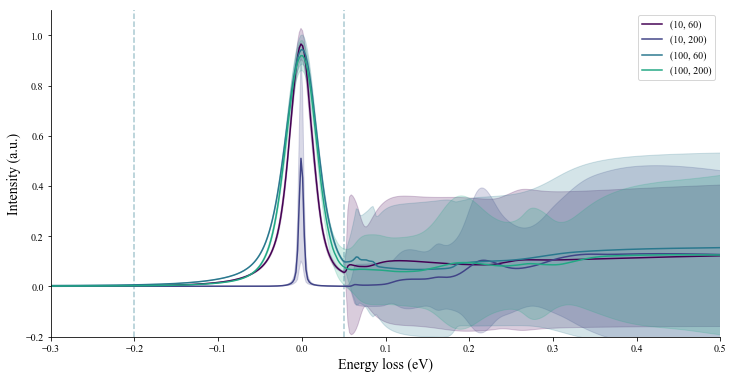
\includegraphics[width=120mm]{plots/extrapolate_energyloss.png}
    \caption{Energy loss extrapolation on vacuum peaks under four different recording settings (exposure time, beam energy). The data within the energy region [-.2, 0.05] eV is known to the network by training. Extrapolation predictions are shown outside this region, marked by the dashed lines.}
    \label{fig:extrapoleloss}
\end{figure}

The goodness of our prediction can be quantified by means of $\chi^2$. So one can separate the parameter space (in Texp and Ebeam for example) into "training" and "prediction" regions, and use one to predict the other. If our error estimate is good, we should find chi2/ndat \simeq 1 also for the predicted datasets


\subsubsection{Beam energy}
\label{sec:ebeam}
The training data contained only two recorded beam energies of 60 and 200 keV. Interpolation and extrapolation predictions have been retrieved on a continuous set of beam energies between 0 and 300 keV. In Fig.~\ref{fig:extrapolbeam} one can observe the mean predicted intensity and mean prediction error, where the average is taken over the energy loss range. The dashed lines indicate the beam energies for which we have data: correspondingly, the errors in these points are small, as the model can make an accurate prediction. The more the beam energy deviates from the known values, the bigger the uncertainties in the predictions become. 

\begin{figure}[H]
    \centering
    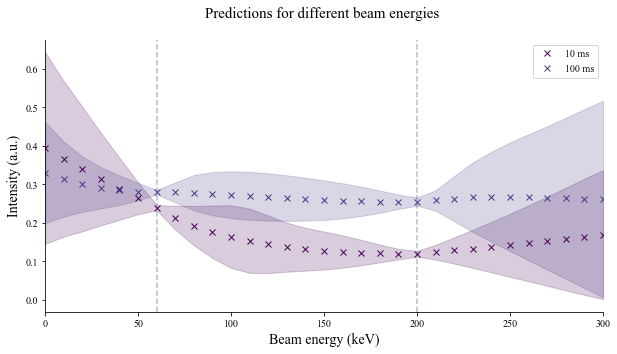
\includegraphics[width=120mm]{plots/Extrapolate_beamenergy.png}
    \caption{Predictions on a continuous set of beam energies, while inputs for energy loss and exposure time are the same as for the training data. The dashed lines indicate the beam energies that are known to the network by training.}
    \label{fig:extrapolbeam}
\end{figure}

\subsubsection{Exposure time}
\label{sec:texp}
The network was trained on data with exposure times of $10$ and $100$ ms, so interpolation and extrapolation is possible. Similar to the predictions for varying beam energy, also for exposure time the uncertainties grow bigger as the value deviates more from the training inputs.

\begin{figure}[H]
    \centering
    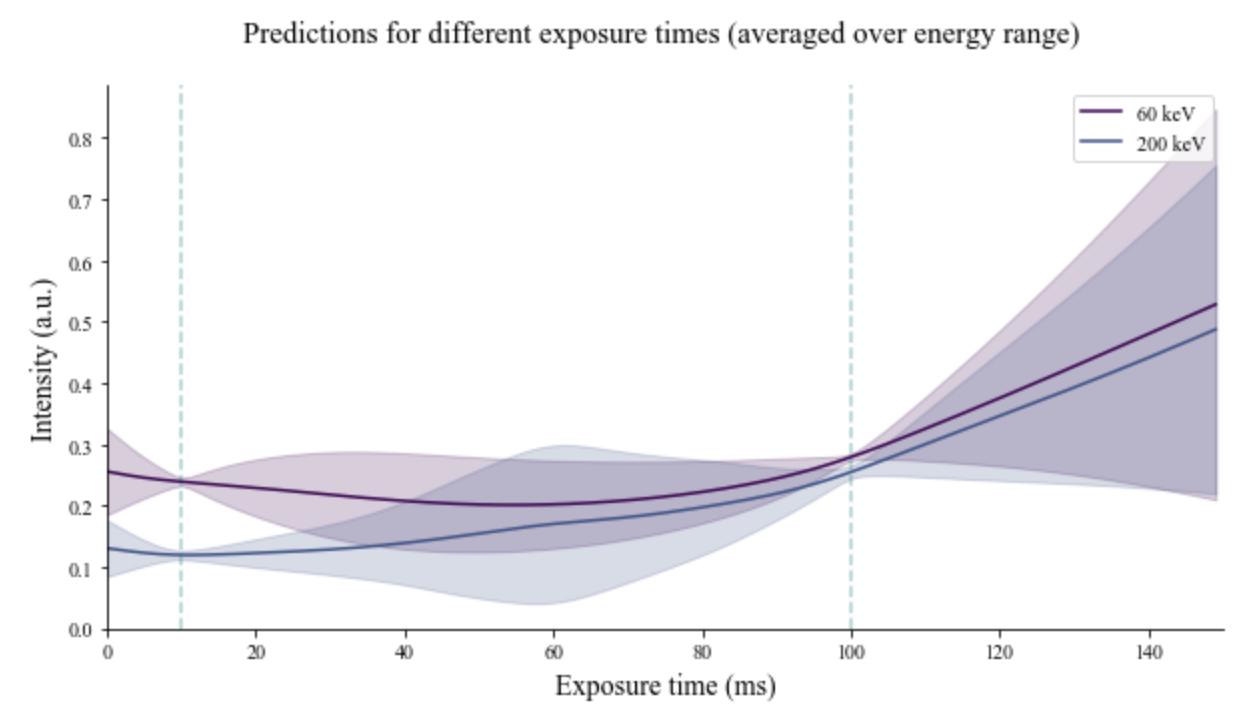
\includegraphics[width=120mm]{plots/Extrapolate_exposuretime.png}
    \caption{Predictions on a continuous set of exposure time, while inputs for energy loss and beam energy are the same as for the training data. The dashed lines indicate the exposure times known to the network by training.}
    \label{fig:extrapolbeam}
\end{figure}

\subsubsection{Fixed energy loss, variable $t_{exp}$ and $E_{beam}$ }
\label{sec:both}



\subsubsection{}



\subsection{Band-gap determination}

Traditionally, bandgaps of dielectrics have been measured by methods offering high energy resolution, however limited spatial resolution~\cite{Park:2008}. Attaching electron monochromators to transmission electron microscopes has proven to be a powerful method for obtaining high spatial resolution, although still limited by the beam size and delocalization phenomena. 

As suggested in literature~\cite{15,14}, the threshold for bandgap detection is the Kimoto limit, which is the energy loss at which 1/1000th of the maximum peak intensity is measured: at this level, sample contributions can be detected above the background of the tails of the zero-loss distribution. We should make sure that we are working above this limit, which for our dataset corresponds to (...) eV.\\

Once the subtracted spectra have been obtained, one can estimate the bandgap, to a first approximation, as the inflection point of the rising intensity. The value can also be roughly estimated from the onset of the absorption or from a linear fit to the maximum positive slope in the EELS spectrum~\cite{Schamm:2003}. However, a more accurate and reliable determination is based on the work of Rafferty and Brown~\cite{Rafferty:2000}. The onset of the subtracted spectrum for a a meterial with a direct bandgap is expected to follow a function of the type
\begin{equation} \label{eq:I1}
    I(E) = I_0 + c\cdot(dE-E_{BG})^{(1/2)}
\end{equation}
where $I_0$ and c are constants, $dE$ is the energy loss and $E_{BG}$ is the bandgap energy. For an indirect bandgap, the power of $(1/2)$ changes to $(3/2)$. Therefore, the bandgap nature (direct or indirect) can be extracted by least-squares fitting of each $(k)$-th replica subtracted spectrum to equation~\ref{eq:I3}:
\begin{equation} \label{eq:I3}
    I(E) = I_0 + c\cdot(dE-E_{BG})^{(b)}.
\end{equation}
This way, by summation over all replicas $N_{rep}$, we can determine the expectation value $\textless{b}\textgreater{}$ and its uncertainty $\sigma_b$. One has to take into account that this approach is very sensitive to the subtraction procedure: the free parameter $E_{BG}$ is the onset of the subtracted spectrum intensity, and it should be investigated how the choice of $dE_1$ affects the free parameter $E_{BG}$.

